\chapter{KHẢO SÁT ĐẶC TUYẾN CỦA LỰC KẾ DỰA TRÊN NGUYÊN TẮC BIẾN DẠNG}

\section{Mục đích thí nghiệm}
\begin{itemize}
	\item Nắm được đặc điểm và kết cấu của dụng cụ đo biến dạng loại lực kế vòng.
	\item Xây dựng được đường đặc tuyến thuận nghịch, mối quan hệ giữa tải trọng và chuyển vị của dụng cụ.
\end{itemize}

\section{Các dụng cụ}
Đồng hồ so loại 0.01mm gắn với biến dạng kế; vòng biến dạng loại 50kg; cân lực để tạo tải trọng $ 0\div 160 $ kg.

\section{Các bước tiến hành}

\begin{table}[ht]
	\centering
	\caption{Bảng đo độ dài theo chiều tăng giảm lực bằng đồng hồ so 0.01mm}
	\begin{tabular}{llllllll}\toprule
		\multirow{2}{*}{STT} & \multirow{2}{*}{Mức lực} & \multicolumn{3}{c}{Chiều tăng lực} & \multicolumn{3}{c}{Chiều giảm lực} \\\cmidrule(r{4pt}){3-5}\cmidrule(r{4pt}){6-8}
		& & Lần 1 & Lần 2 & Lần 3 &  Lần 1 & Lần 2 & Lần 3 \\\midrule
		1 & 10 & 1 & 3 & 2 & 3 & 2 & 2\\
		2 & 20 & 5 & 5 & 4 & 6 & 5 & 4\\
		3 & 30 & 8 & 8 & 7 & 8 & 8 & 7\\
		4 & 40 & 10 & 10 & 9 & 11 & 10 & 9 \\
		5 & 50 & 12 & 13 & 11 & 13 & 11 & 10\\
		6 & 60 & 15 & 15 & 13 & 13 & 13 & 14\\
		7 & 70 & 17 & 17 & 16 & 18 & 19 & 16\\
		8 & 80 & 20 & 20 & 19 & 20 & 20 & 19\\
		9 & 90 & 22 & 22 & 20 & 22 & 21 & 21\\
		10 & 100 & 25 & 23 & 23 & 25 & 25 & 23\\\bottomrule
	\end{tabular}
\end{table}

\section{Đánh giá kết quả}
\begin{figure}[ht]
	\centering
	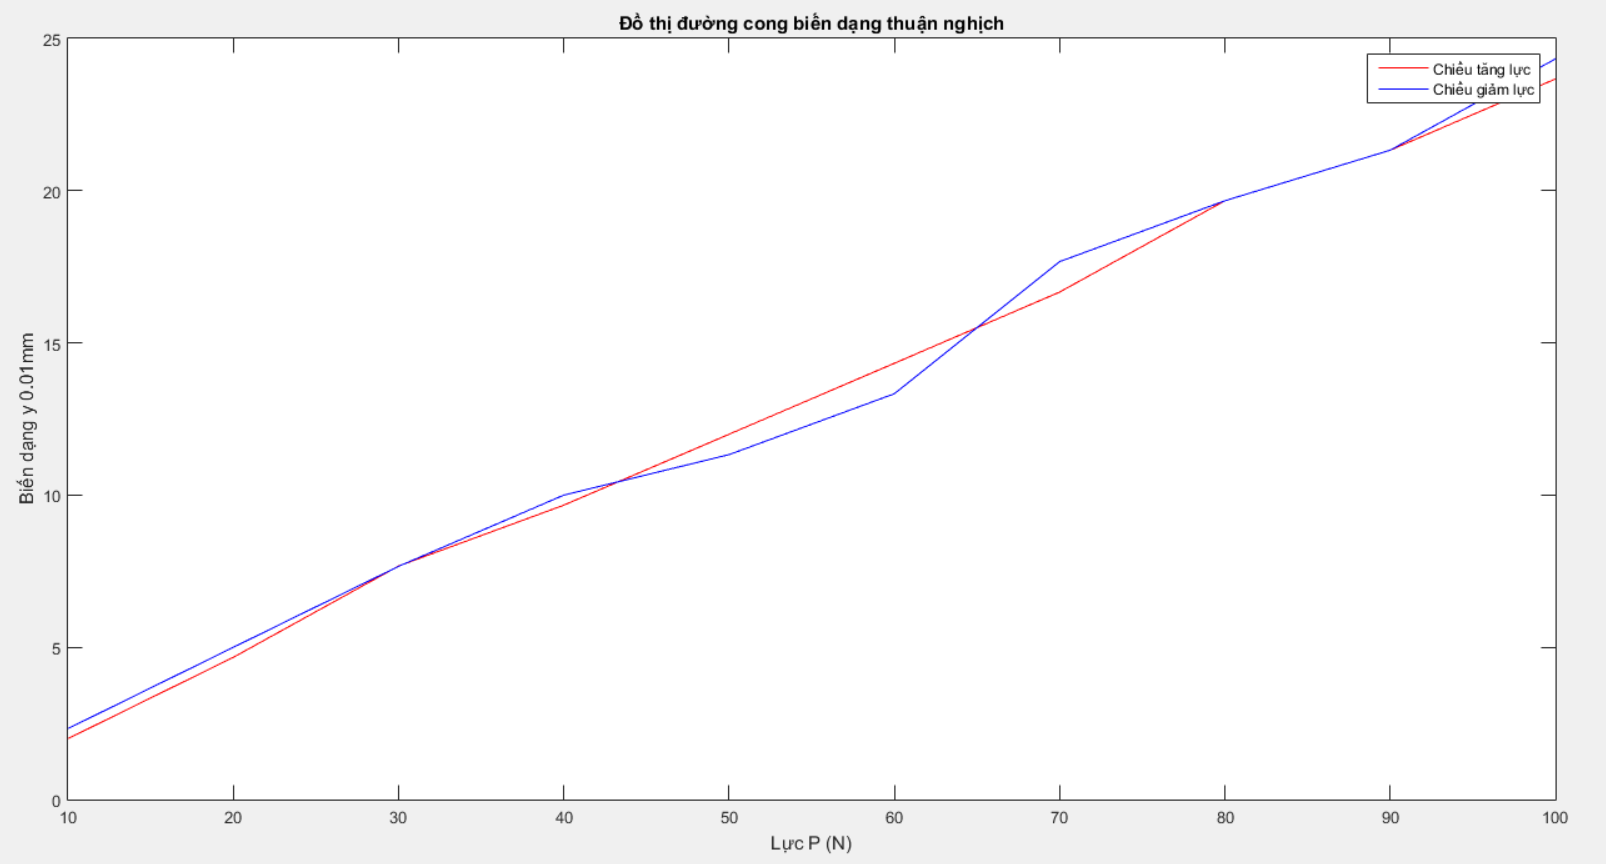
\includegraphics[width=.75\linewidth]{screenshot001}
	\caption{Đồ thị đường cong biến dạng thuận nghịch}
\end{figure}
Kết quả đo khá chính xác vì:
\begin{itemize}
	\item Sử dụng thước panme chuyên dụng có độ chính xác cao.
	\item Đo theo nguyên tắc ABBE.
\end{itemize}
Dung sai độ dao động khoảng pháp tuyến chung dùng để đánh giá mức độ chính xác động học của bánh răng.

Nhận xét:
\begin{itemize}
	\item Đường cong biến dạng thuận có dạng tuyến tính (gần đúng).
	\item Đường cong biến dạng nghịch có dạng tuyến tính (gần đúng).
	\item Hai đường cong này không trùng nhau.
\end{itemize}

Xác định độ cứng của của vòng biến dạng: $ J = P/y $. Do đường cong khi tăng tải và giảm tải không trùng nhau nên để đánh giá độ cứng vững của vòng biến dạng, ta hình dung độ cứng vững trung bình và đường cong biến dạng lúc này được chọn là đường thẳng sao cho diện tích ở 2 phía đường cong như sau:
\[
J = P/y = \dfrac{100-10}{(24.33-2.33)\times 10^{-2}} = 409.1 \unitp{N/mm}
\]